\section{przypadek testowy 5}
\subsection{Cel: }
Celem badania jest sprawdzenie jak dokładne są rozwiązania metodą two-opt dla instancji testowych problemów symetrycznych i asymetrycznych z \href{http://comopt.ifi.uni-heidelberg.de/software/TSPLIB95/}{TSPLIB}.
\subsection{Założenia: }
Podczas badania korzystać będziemy z wybranych instancji symetrycznych oraz asymetrycznych z biblioteki TSPLIB w trzech formatach danych FULL MATRIX, LOWER DIAG ROW i EUC 2D. Najlepszym wynikiem - referencyjnym będziemy określać najmniejszą długość ścieżki w grafie wyznaczoną przez jedną z trzech algorytmów: k-random, nearest-neighbor, two-opt.

\subsection{Wyniki: }
\begin{table}[H]
  \centering
  \begin{tabular}{|l|l|l|l|}
  \hline
      instance name & two-opt cost & reference cost & PRD \\ \hline \hline
      a280.tsp & 2715 & 2715 & 0 \\ \hline
      bays29.tsp & 2108 & 2108 & 0 \\ \hline
      berlin52.tsp & 8384 & 8384 & 0 \\ \hline
      bier127.tsp & 123545 & 123545 & 0 \\ \hline
      ch130.tsp & 6457 & 6457 & 0 \\ \hline
      ch150.tsp & 7056 & 7053 & 0.042535091 \\ \hline
      d198.tsp & 16340 & 16340 & 0 \\ \hline
      d493.tsp & 37645 & 37645 & 0 \\ \hline
      dantzig42.tsp & 699 & 699 & 0 \\ \hline
      eil51.tsp & 443 & 443 & 0 \\ \hline
      eil76.tsp & 570 & 570 & 0 \\ \hline
      eil101.tsp & 662 & 662 & 0 \\ \hline
      fl417.tsp & 12188 & 12188 & 0 \\ \hline
      fri26.tsp & 937 & 937 & 0 \\ \hline
      gil262.tsp & 2601 & 2601 & 0 \\ \hline
      gr17.tsp & 2211 & 2211 & 0 \\ \hline
      gr21.tsp & 2801 & 2801 & 0 \\ \hline
      gr24.tsp & 1278 & 1278 & 0 \\ \hline
      gr48.tsp & 5278 & 5278 & 0 \\ \hline
      gr120.tsp & 7390 & 7390 & 0 \\ \hline
      hk48.tsp & 11718 & 11718 & 0 \\ \hline
      kroA100.tsp & 22883 & 22883 & 0 \\ \hline
      kroA150.tsp & 28600 & 28600 & 0 \\ \hline
      kroA200.tsp & 31148 & 31148 & 0 \\ \hline
      kroB100.tsp & 23134 & 23134 & 0 \\ \hline
      kroB150.tsp & 28223 & 28223 & 0 \\ \hline
      kroB200.tsp & 31767 & 31767 & 0 \\ \hline
      kroC100.tsp & 22727 & 22727 & 0 \\ \hline
      kroD100.tsp & 23218 & 23218 & 0 \\ \hline
      lin105.tsp & 14941 & 14941 & 0 \\ \hline
      lin318.tsp & 45721 & 45721 & 0 \\ \hline
      pr76.tsp & 121207 & 121207 & 0 \\ \hline
      pr107.tsp & 47691 & 46927 & 1.628060605 \\ \hline
      pr124.tsp & 63212 & 63212 & 0 \\ \hline
      pr136.tsp & 99770 & 99770 & 0 \\ \hline
      pr144.tsp & 58796 & 58796 & 0 \\ \hline
      pr152.tsp & 75662 & 75662 & 0 \\ \hline
  \end{tabular}
  \caption{TSP}
\end{table}

\begin{table}[H]
  \centering
  \begin{tabular}{|l|l|l|l|}
  \hline
      instance name & two-opt cost & reference cost & PRD \\ \hline \hline
      br17.atsp & 39 & 39 & 0 \\ \hline
      ft53.atsp & 8657 & 8657 & 0 \\ \hline
      ft70.atsp & 44669 & 43264 & 3.247503698 \\ \hline
      ftv170.atsp & 5140 & 3959 & 29.83076534 \\ \hline
      ftv33.atsp & 2036 & 1664 & 22.35576923 \\ \hline
      ftv35.atsp & 2245 & 1869 & 20.11771001 \\ \hline
      ftv38.atsp & 2264 & 1830 & 23.71584699 \\ \hline
      ftv44.atsp & 2522 & 1884 & 33.8641189 \\ \hline
      ftv47.atsp & 3136 & 2338 & 34.13173653 \\ \hline
      ftv55.atsp & 2907 & 2344 & 24.01877133 \\ \hline
      ftv64.atsp & 4173 & 2629 & 58.72955496 \\ \hline
      ftv70.atsp & 3434 & 2715 & 26.4825046 \\ \hline
      kro124p.atsp & 52705 & 44612 & 18.14085896 \\ \hline
      p43.atsp & 5638 & 1023 & 451.1241447 \\ \hline
      rbg323.atsp & 4251 & 1742 & 144.0298507 \\ \hline
      rbg358.atsp & 4649 & 1806 & 157.4197121 \\ \hline
      rbg403.atsp & 5207 & 3543 & 46.96584815 \\ \hline
      rbg443.atsp & 5897 & 3913 & 50.70278559 \\ \hline
      ry48p.atsp & 15965 & 15965 & 0 \\ \hline
  \end{tabular}
  \caption{aTSP}
\end{table}

W tabelach przedstawione zostały wyniki eksperymentu oraz obliczone na ich podstawie PRD według wzoru \[ PRD_x = 100 \cdot \frac{x - x_{ref}}{x_{ref}}\]

\begin{table}[H]
  \centering
  \begin{tabular}{|l|l|l|}
  \hline
     wariant & tsp & atsp \\ \hline \hline
     średnie PRD & 0.045151235 & 60.25670957 \\ \hline
     odchylenie standardowe & 0.267548599 & 103.9669193 \\ \hline
  \end{tabular}
  \caption{średnie PRD dla obu wariantów}
\end{table}

\subsection{Wykresy: }
\begin{figure}[H]
    \centering
    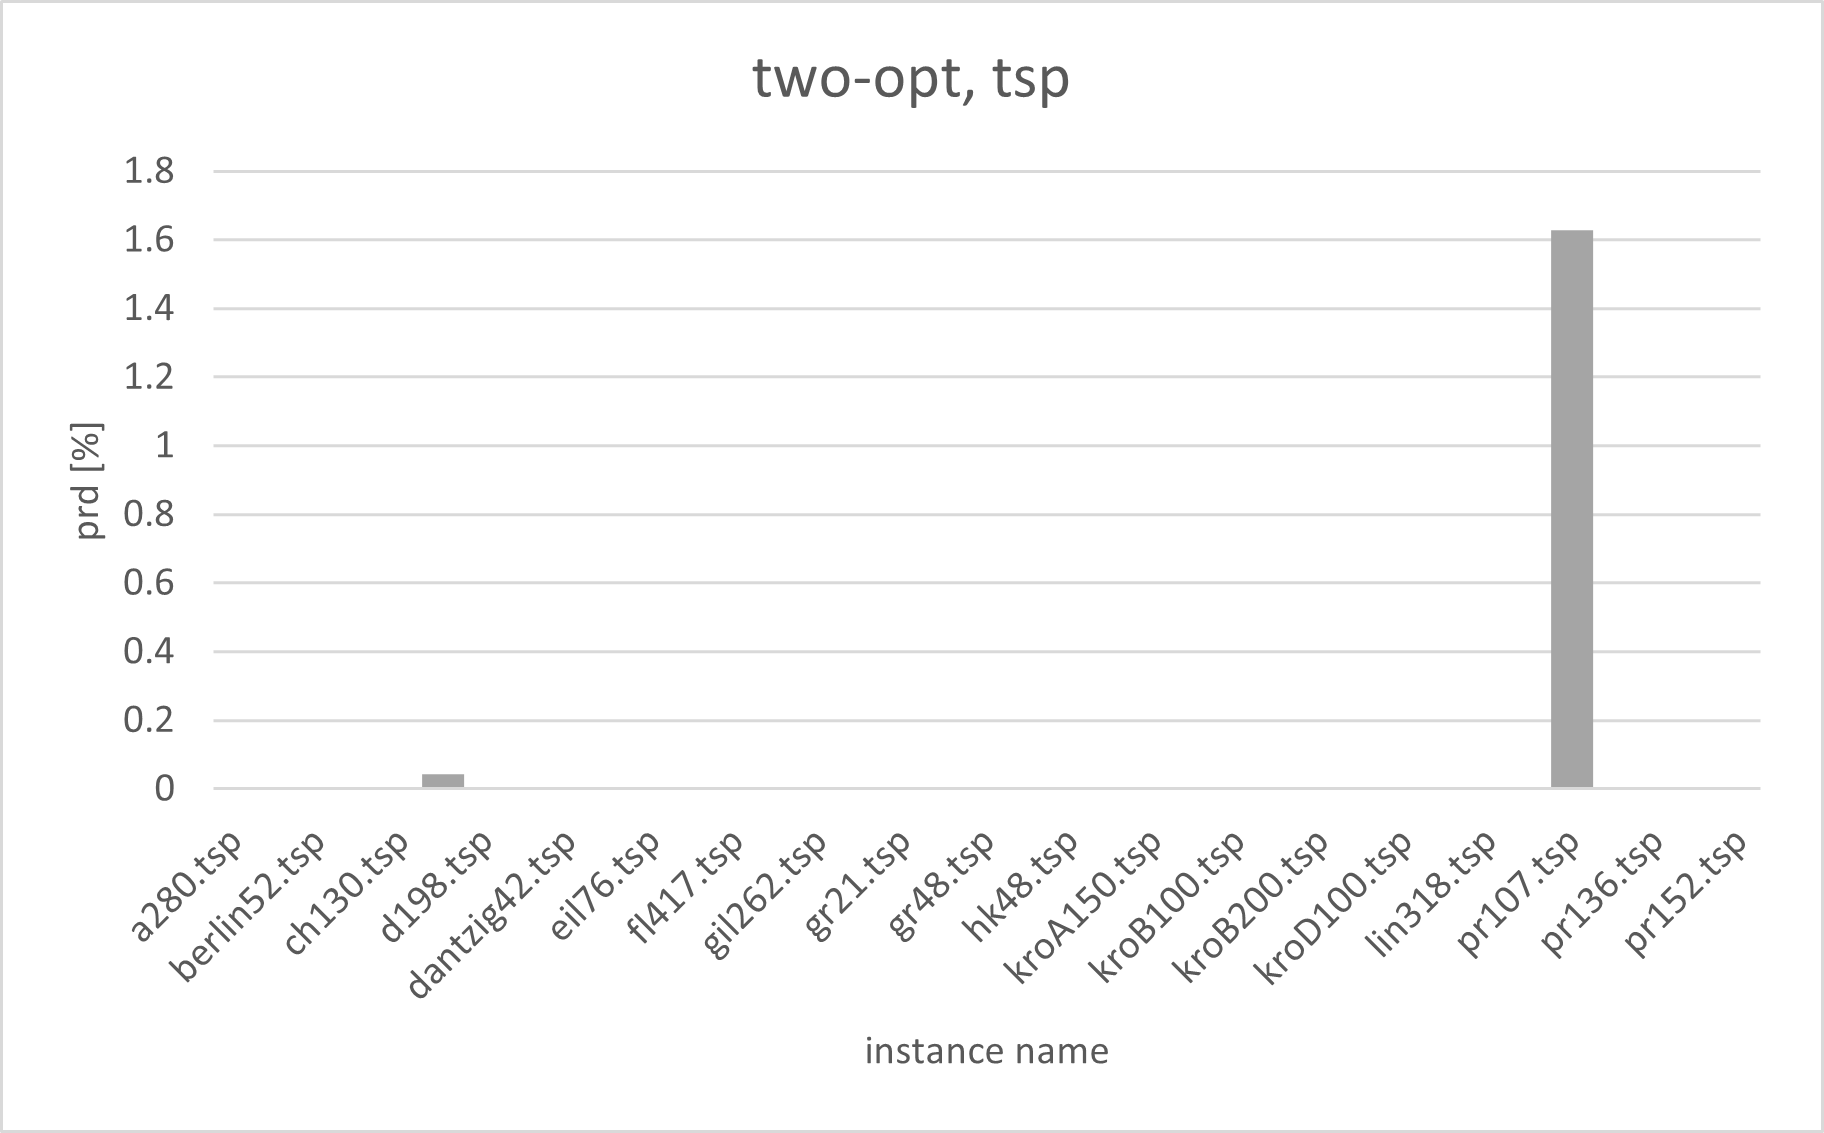
\includegraphics[width=\linewidth]{chart_test4_tsp.png}
    \caption{Wartości PRD dla instancji TSP}
\end{figure}
\begin{figure}[H]
  \centering
  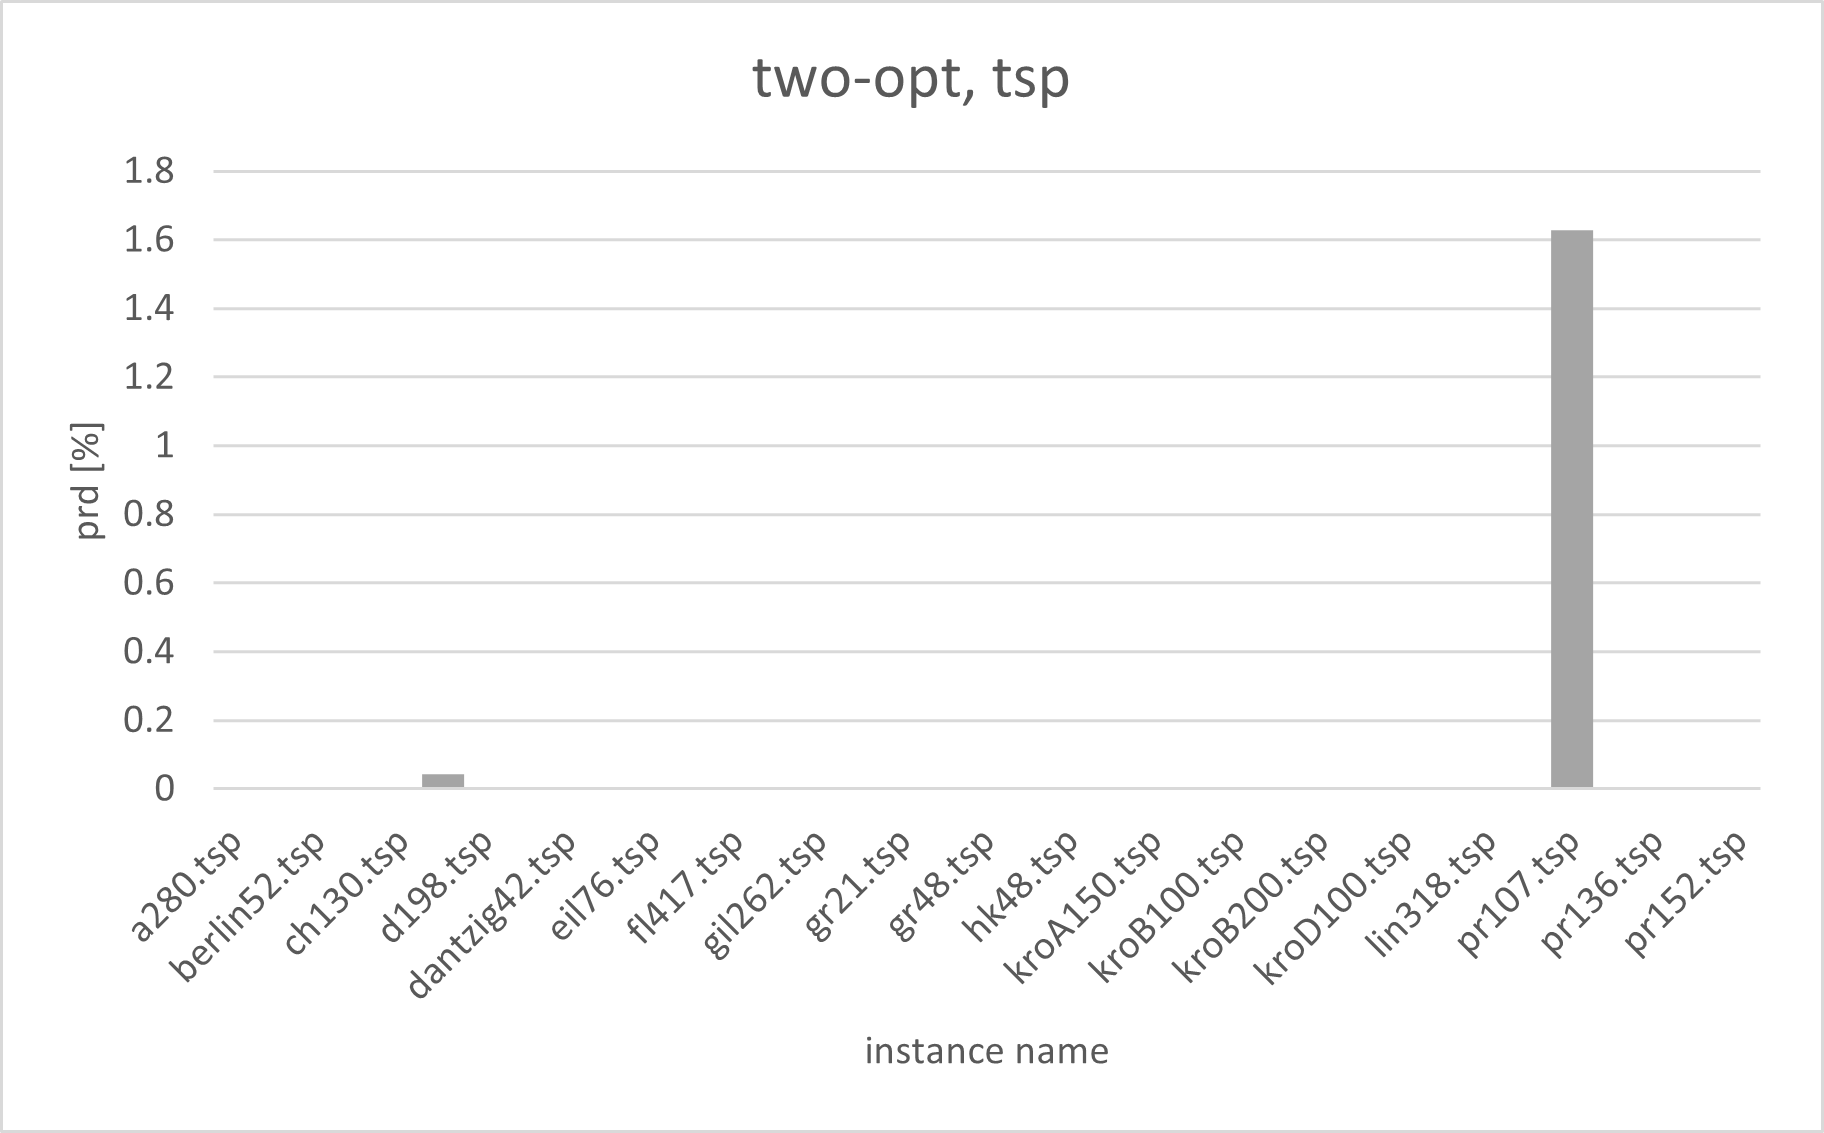
\includegraphics[width=\linewidth]{chart_test4_tsp.png}
  \caption{Wartości PRD dla instancji ATSP}
\end{figure}
Na osi OX wykresu naniesione zostały nazwy instancji dla których wykonywany był pomniar, na osi OY zostały naniesione wartości PRD.

\subsection{Wnioski: }
Uzyskane dane sugerują, że algorytm two-opt dużo lepiej radzi sobie z instancjami symetrycznymi problemów. Otóż może być to część prawdy, gdyż w instancjach asymetrycznych nie są (nie muszą być) zachowane nierówności trójkąta. Z drugiej strony 2 instancje symetryczne w których algorytm nie dał najlepszego znanego wyniku miały postać euklidesową gdzie nierówności trójkąta były zachowane. 

